\section{Inverse Sinusoidal as $f(t)$}
This report analyzes the convolution of the inverse sine function with a rectangular kernel, examining both analytical and numerical approaches. We investigate how system parameters influence the convolution output while addressing the unique challenges posed by the arcsin function's domain constraints and singularities.

\subsection{Mathematical Formulation}

\subsubsection{Convolution Definition}
The convolution of an input signal $f(t)$ with a kernel $h(t)$ is defined as:
\begin{equation}
y(t) = (f * h)(t) = \int_{-\infty}^{\infty} f(\tau)h(t-\tau)d\tau
\end{equation}

For our specific case:
\begin{align}
f(t) &= 
\begin{cases}
A\arcsin(t), & -1 \leq t \leq 1 \\
0, & \text{otherwise}
\end{cases} \\
h(t) &= 
\begin{cases} 
1, & |t| \leq T \\
0, & \text{otherwise}
\end{cases}
\end{align}

\subsubsection{Analytical Solution}
The convolution integral becomes:
\begin{equation}
y(t) = \int_{t-T}^{t+T} A\arcsin(\tau)d\tau
\end{equation}

Using the primitive $\int \arcsin(x)dx = x\arcsin(x) + \sqrt{1-x^2} + C$, we derive the piecewise solution:

\begin{align*}
y(t) &= \begin{cases}
A\left[(t+T)\arcsin(t+T) + \sqrt{1-(t+T)^2}\right. \\
\quad \left.- (t-T)\arcsin(t-T) - \sqrt{1-(t-T)^2}\right], & \text{Case 1: } -1 \leq t-T \leq t+T \leq 1 \\
A\left[(t+T)\arcsin(t+T) + \sqrt{1-(t+T)^2} + \frac{\pi}{2}\right], & \text{Case 2: } t-T < -1 \leq t+T \leq 1 \\
A\left[\frac{\pi}{2} - (t-T)\arcsin(t-T) - \sqrt{1-(t-T)^2}\right], & \text{Case 3: } -1 \leq t-T \leq 1 < t+T \\
A\pi, & \text{Case 4: } t-T < -1 \text{ and } t+T > 1
\end{cases}
\end{align*}

\subsection{Numerical Implementation}
The numerical approach discretizes the convolution integral:
\begin{equation}
y[n] = \Delta t \sum_{k=-N}^{N} f[k]h[n-k]
\end{equation}

Key considerations:
\begin{itemize}
\item Strict domain enforcement for the arcsin function
\item Proper handling of integration limits at domain boundaries
\item Special handling of boundary regions
\end{itemize}

\begin{figure}[H]
    \centering
    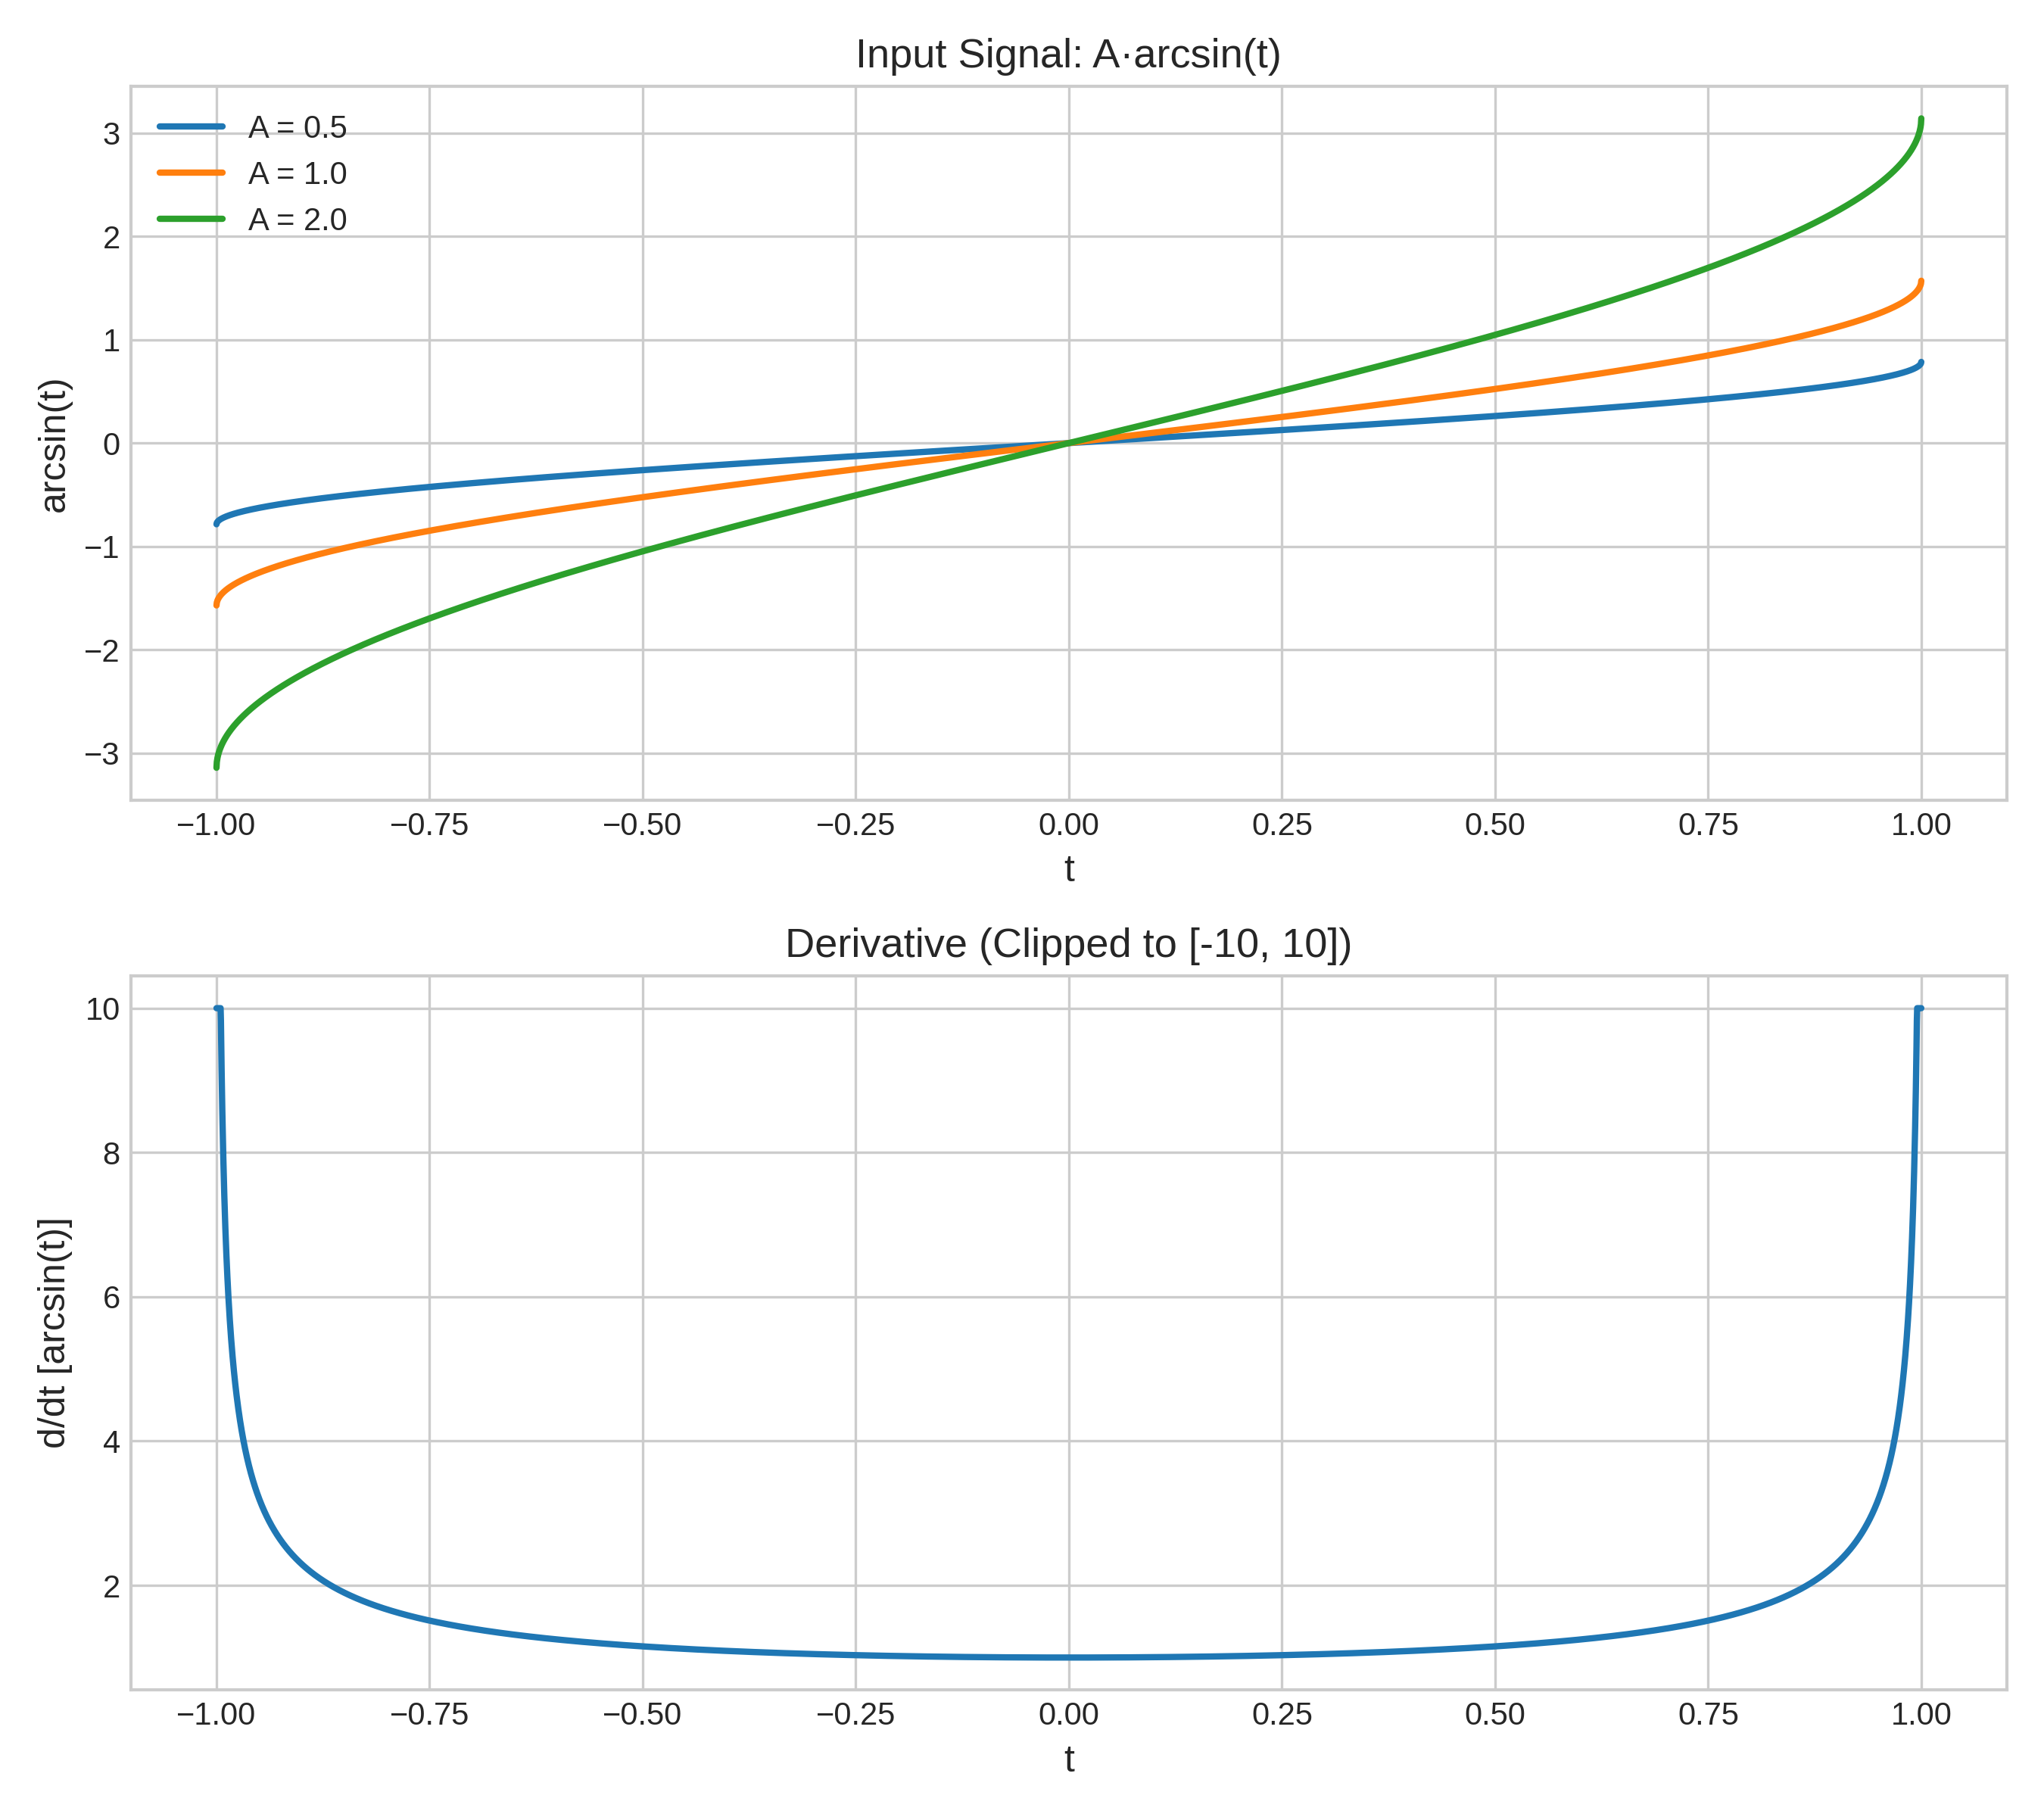
\includegraphics[width=0.85\textwidth]{codes/codes_sin_1_and_arcsin/figures/arcsin_properties.png}
    \caption{Properties of the arcsin function showing (a) amplitude variations and (b) singular derivative at boundaries}
    \label{fig:properties}
\end{figure}

\subsection{Parameter Analysis}

\subsubsection{Amplitude Effects}
\begin{figure}[H]
    \centering
    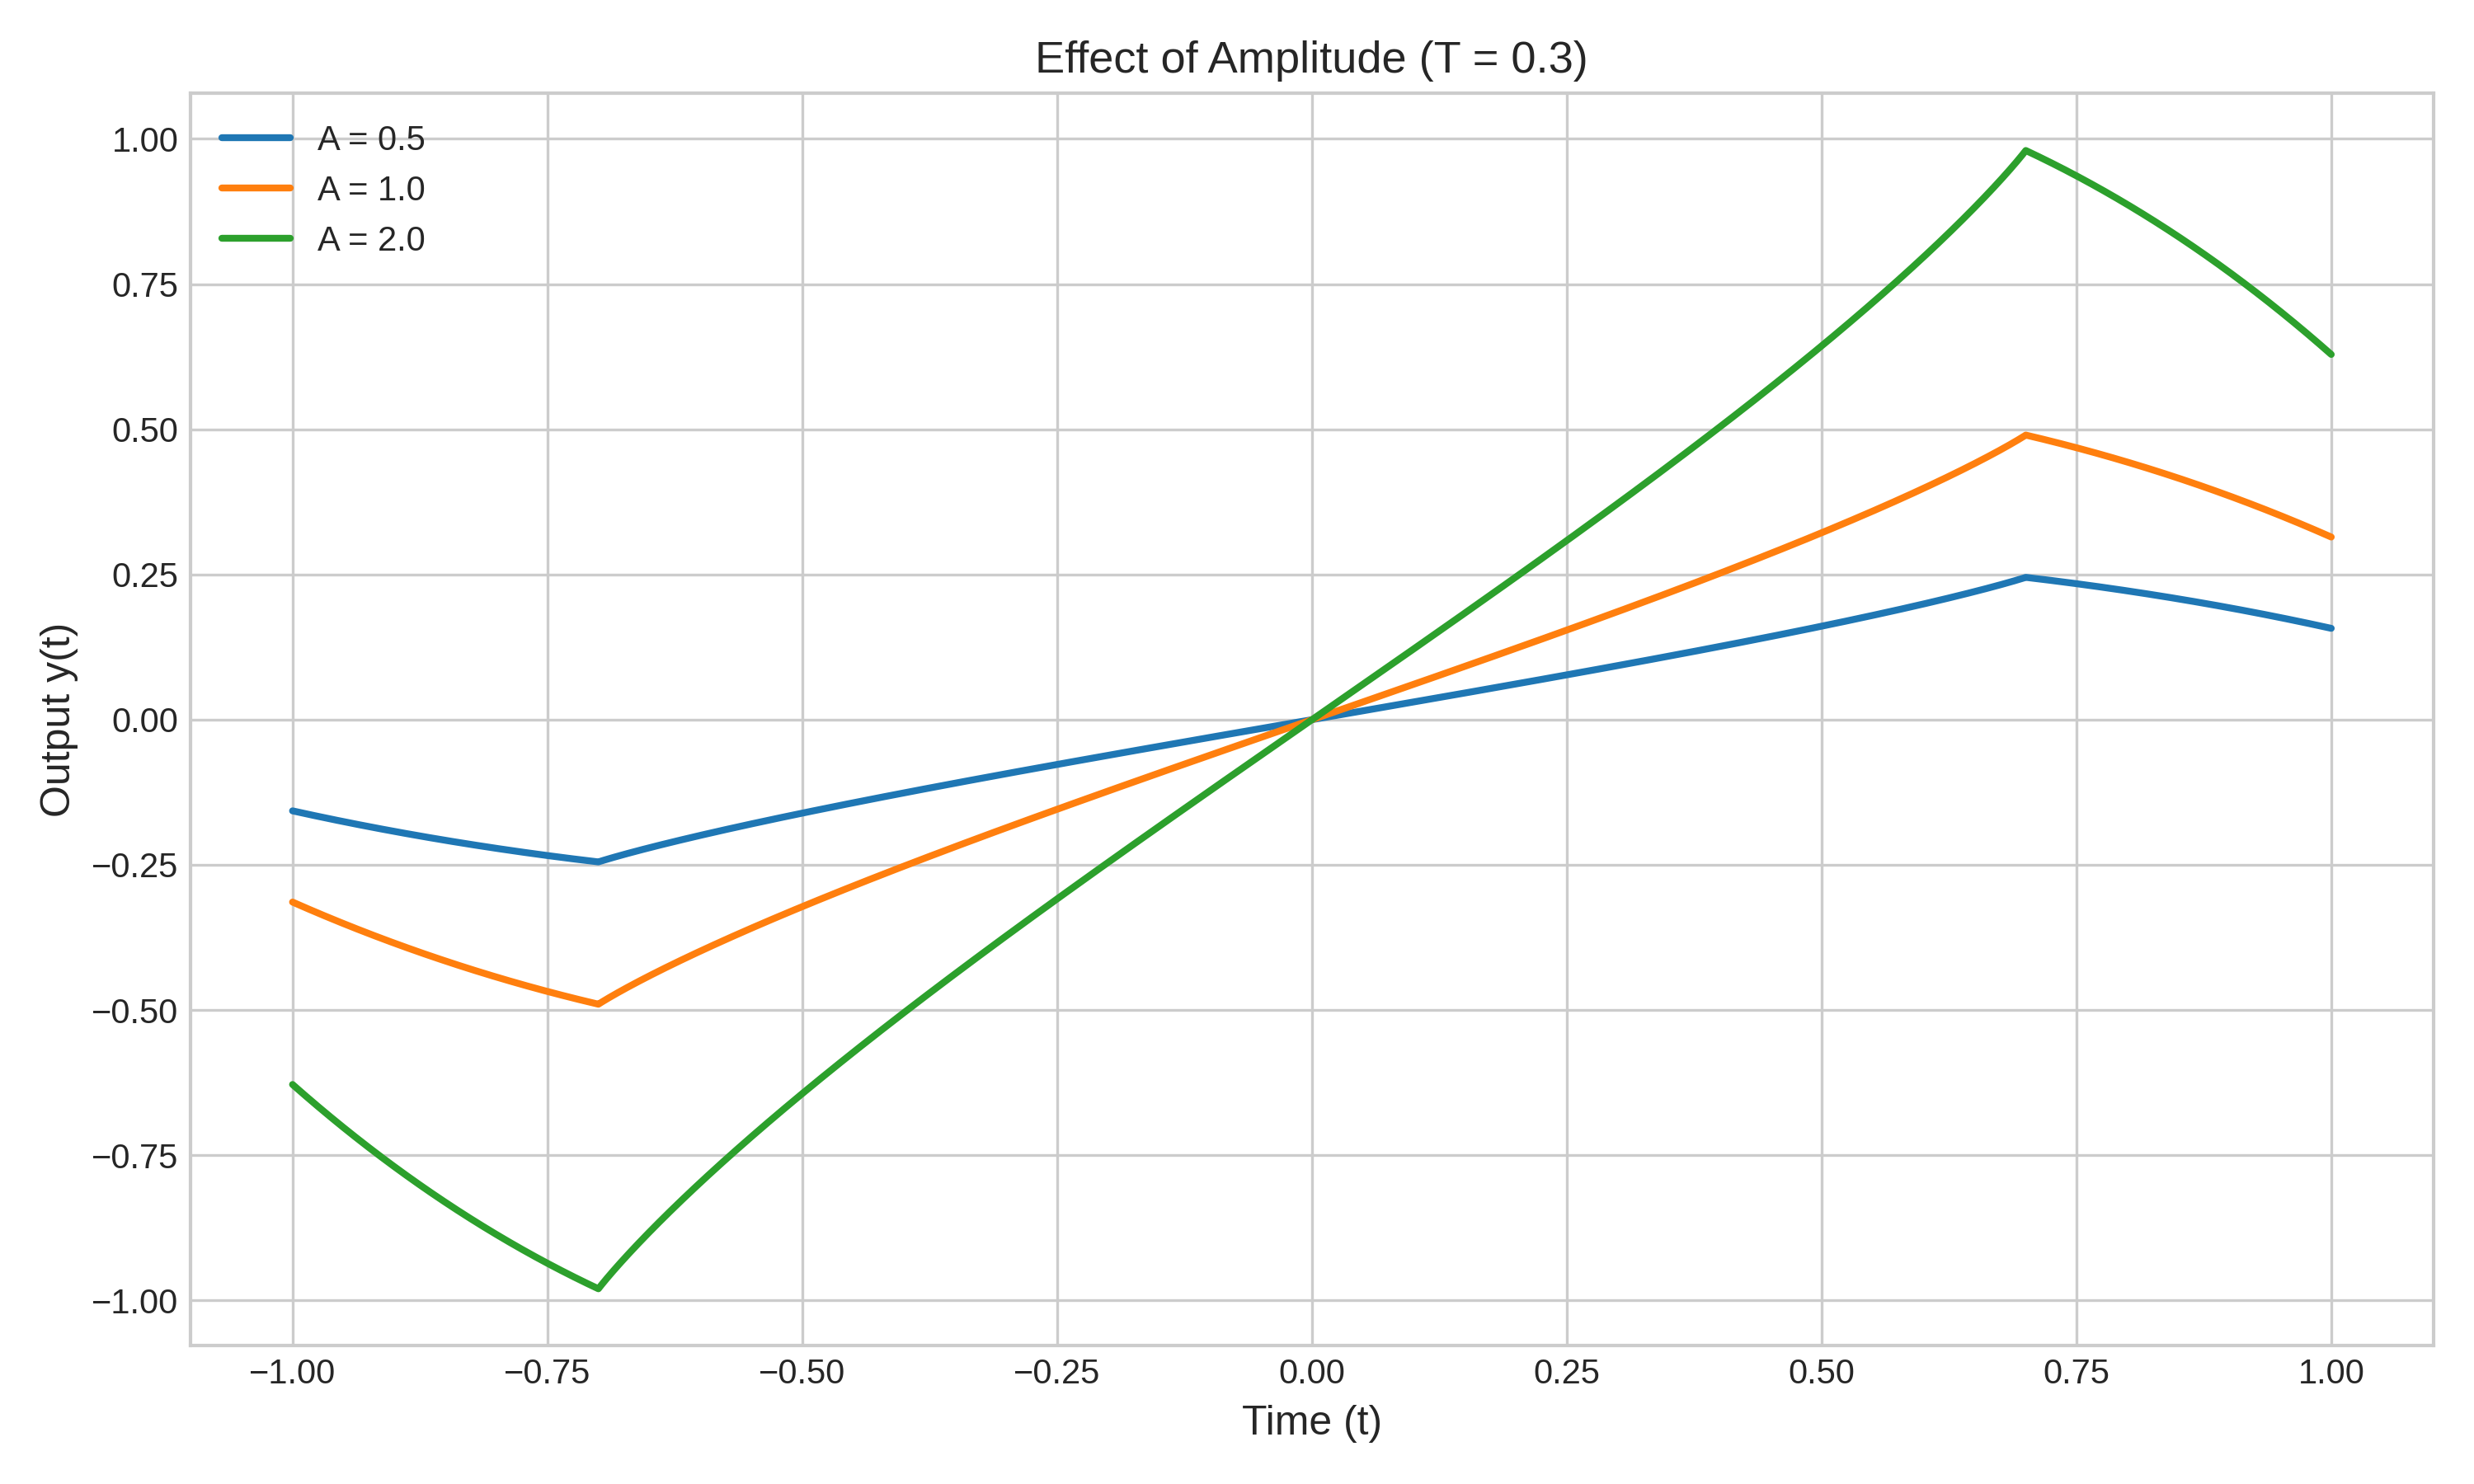
\includegraphics[width=0.85\textwidth]{codes/codes_sin_1_and_arcsin/figures/amplitude_effect.png}
    \caption{Linear scaling of convolution output with amplitude $A$ (kernel width $T=0.3$)}
    \label{fig:amplitude}
\end{figure}

Key observations:
\begin{itemize}
\item Output amplitude scales linearly with $A$
\item Shape preservation demonstrates system linearity
\item Boundary effects remain consistent across amplitudes
\end{itemize}

\subsubsection{Kernel Width Effects}
\begin{figure}[H]
    \centering
    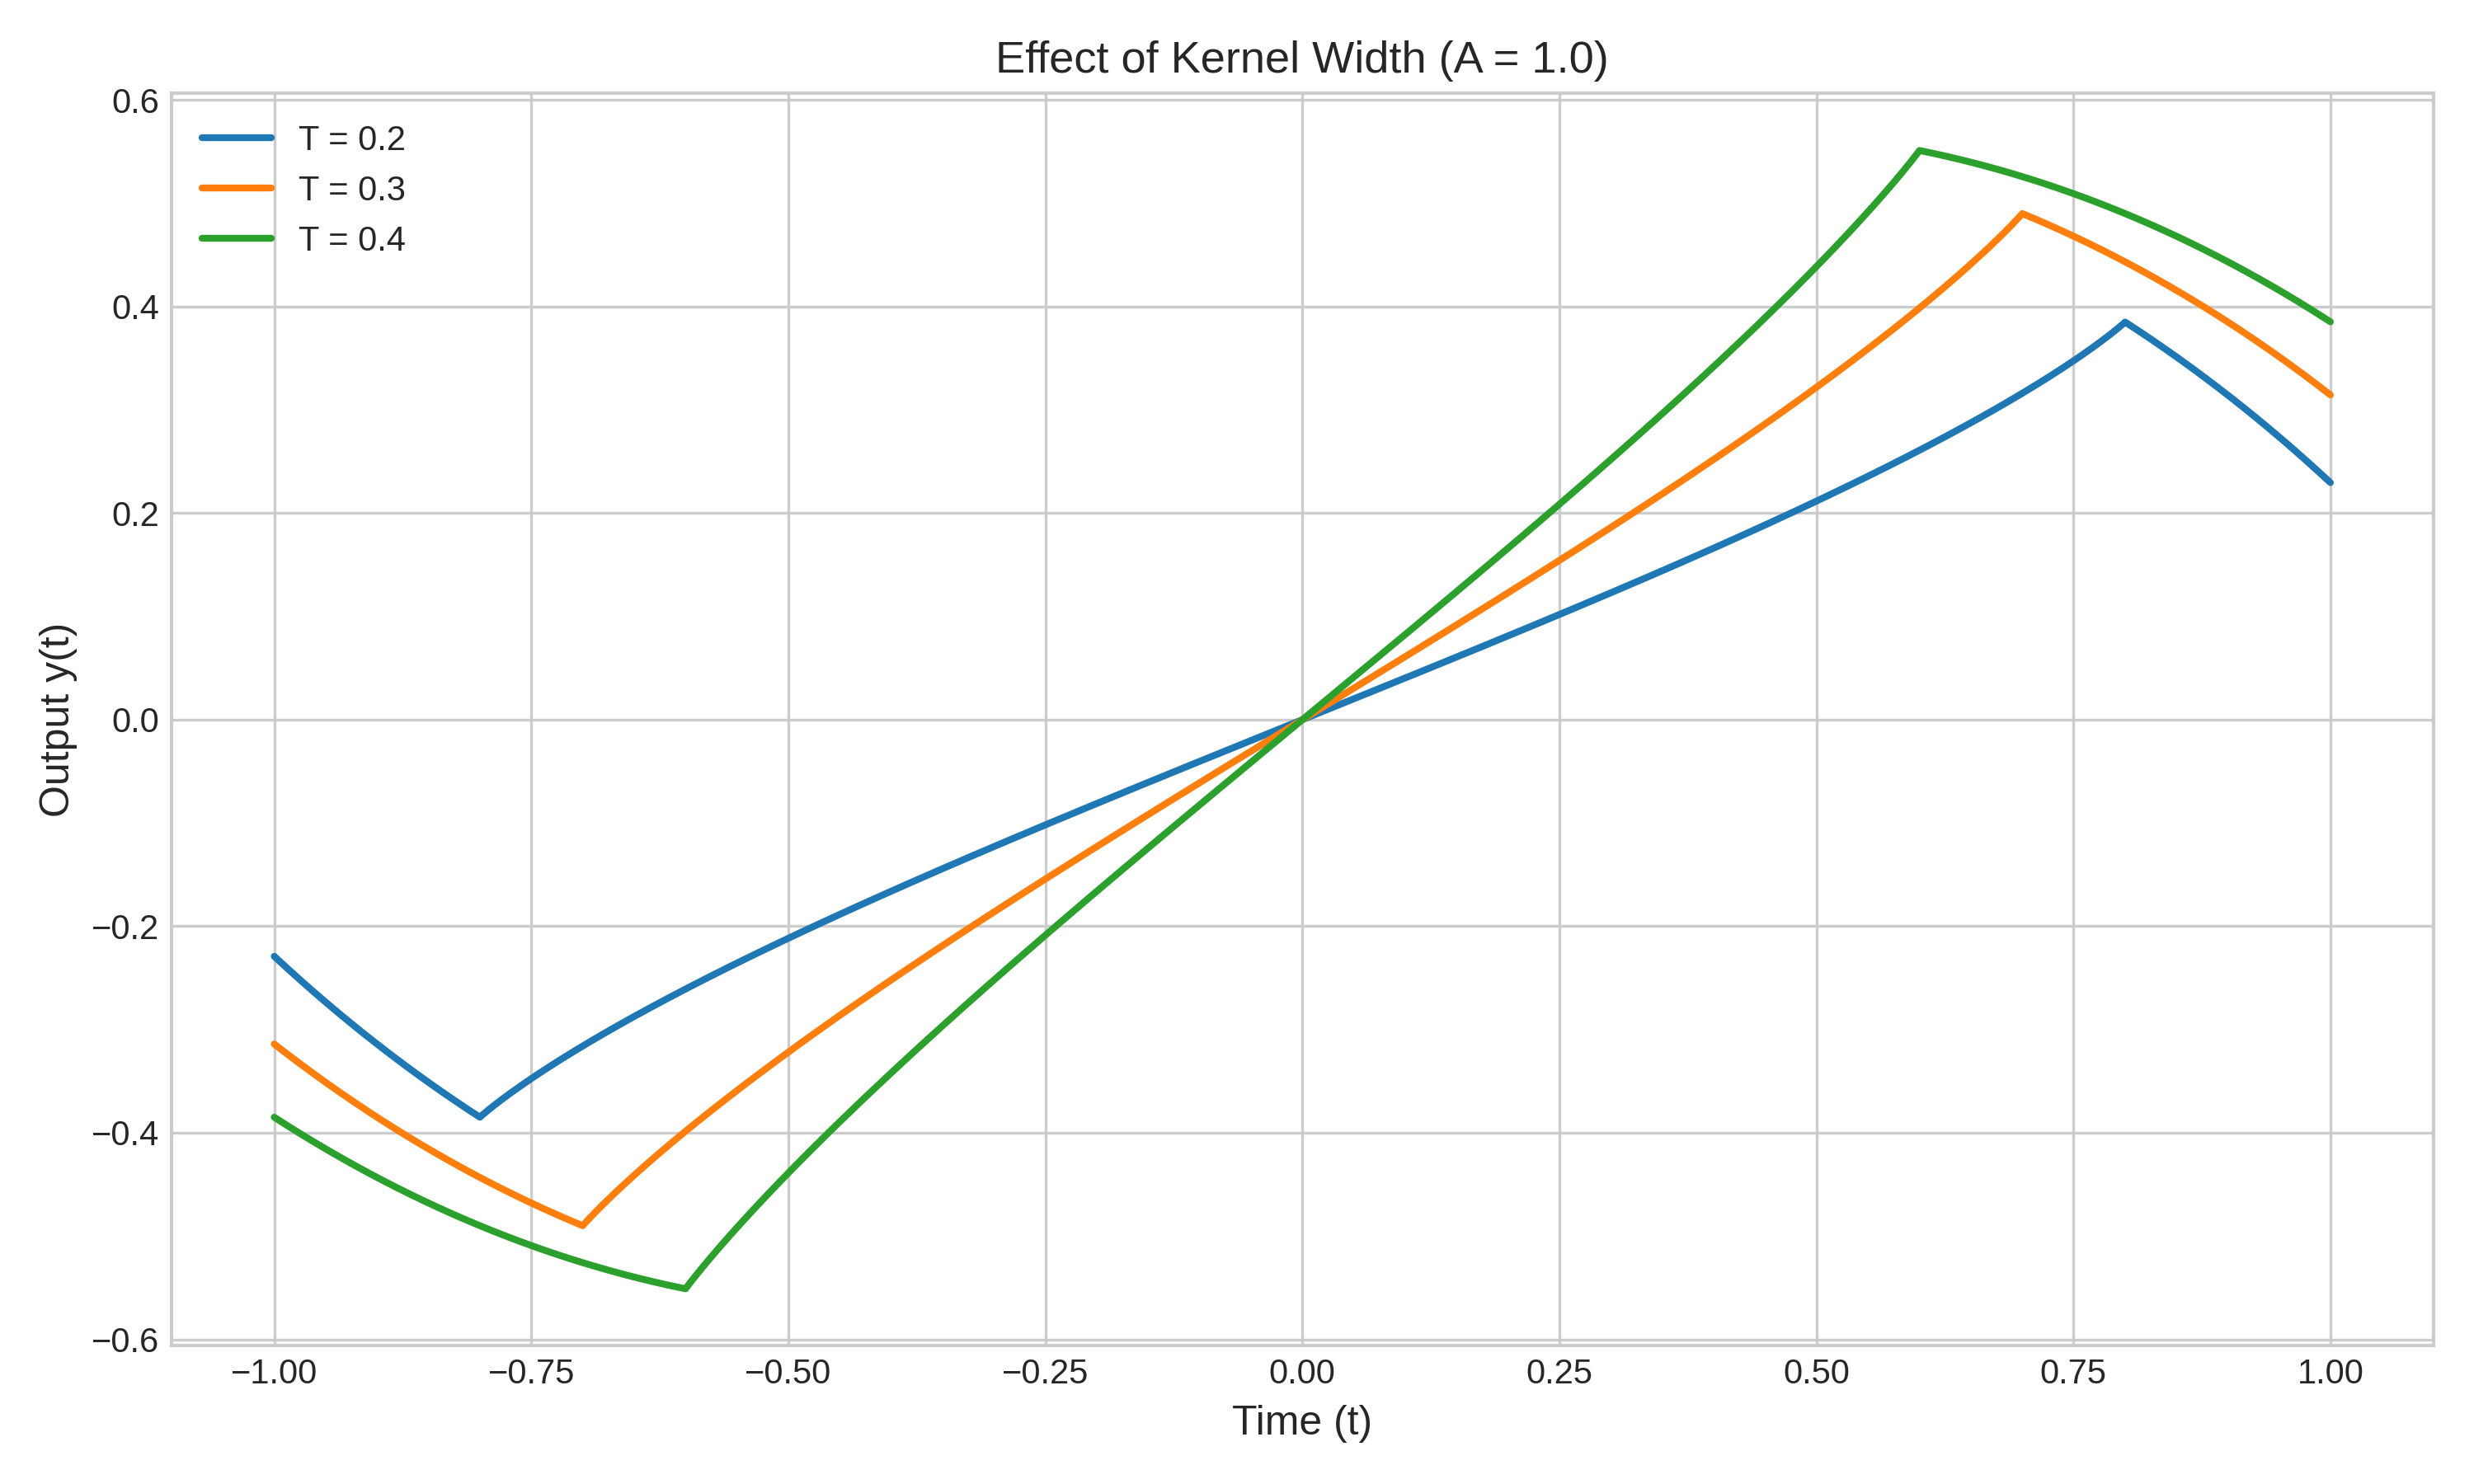
\includegraphics[width=0.85\textwidth]{codes/codes_sin_1_and_arcsin/figures/kernel_width_effect.png}
    \caption{Impact of kernel width $T$ on output smoothing (amplitude $A=1$)}
    \label{fig:kernel}
\end{figure}

Key observations:
\begin{itemize}
\item Wider kernels increase smoothing
\item Output amplitude increases with larger $T$
\item Boundary effects become more pronounced
\end{itemize}

\subsection{System Validation}

\subsubsection{Method Comparison}
\begin{figure}[H]
    \centering
    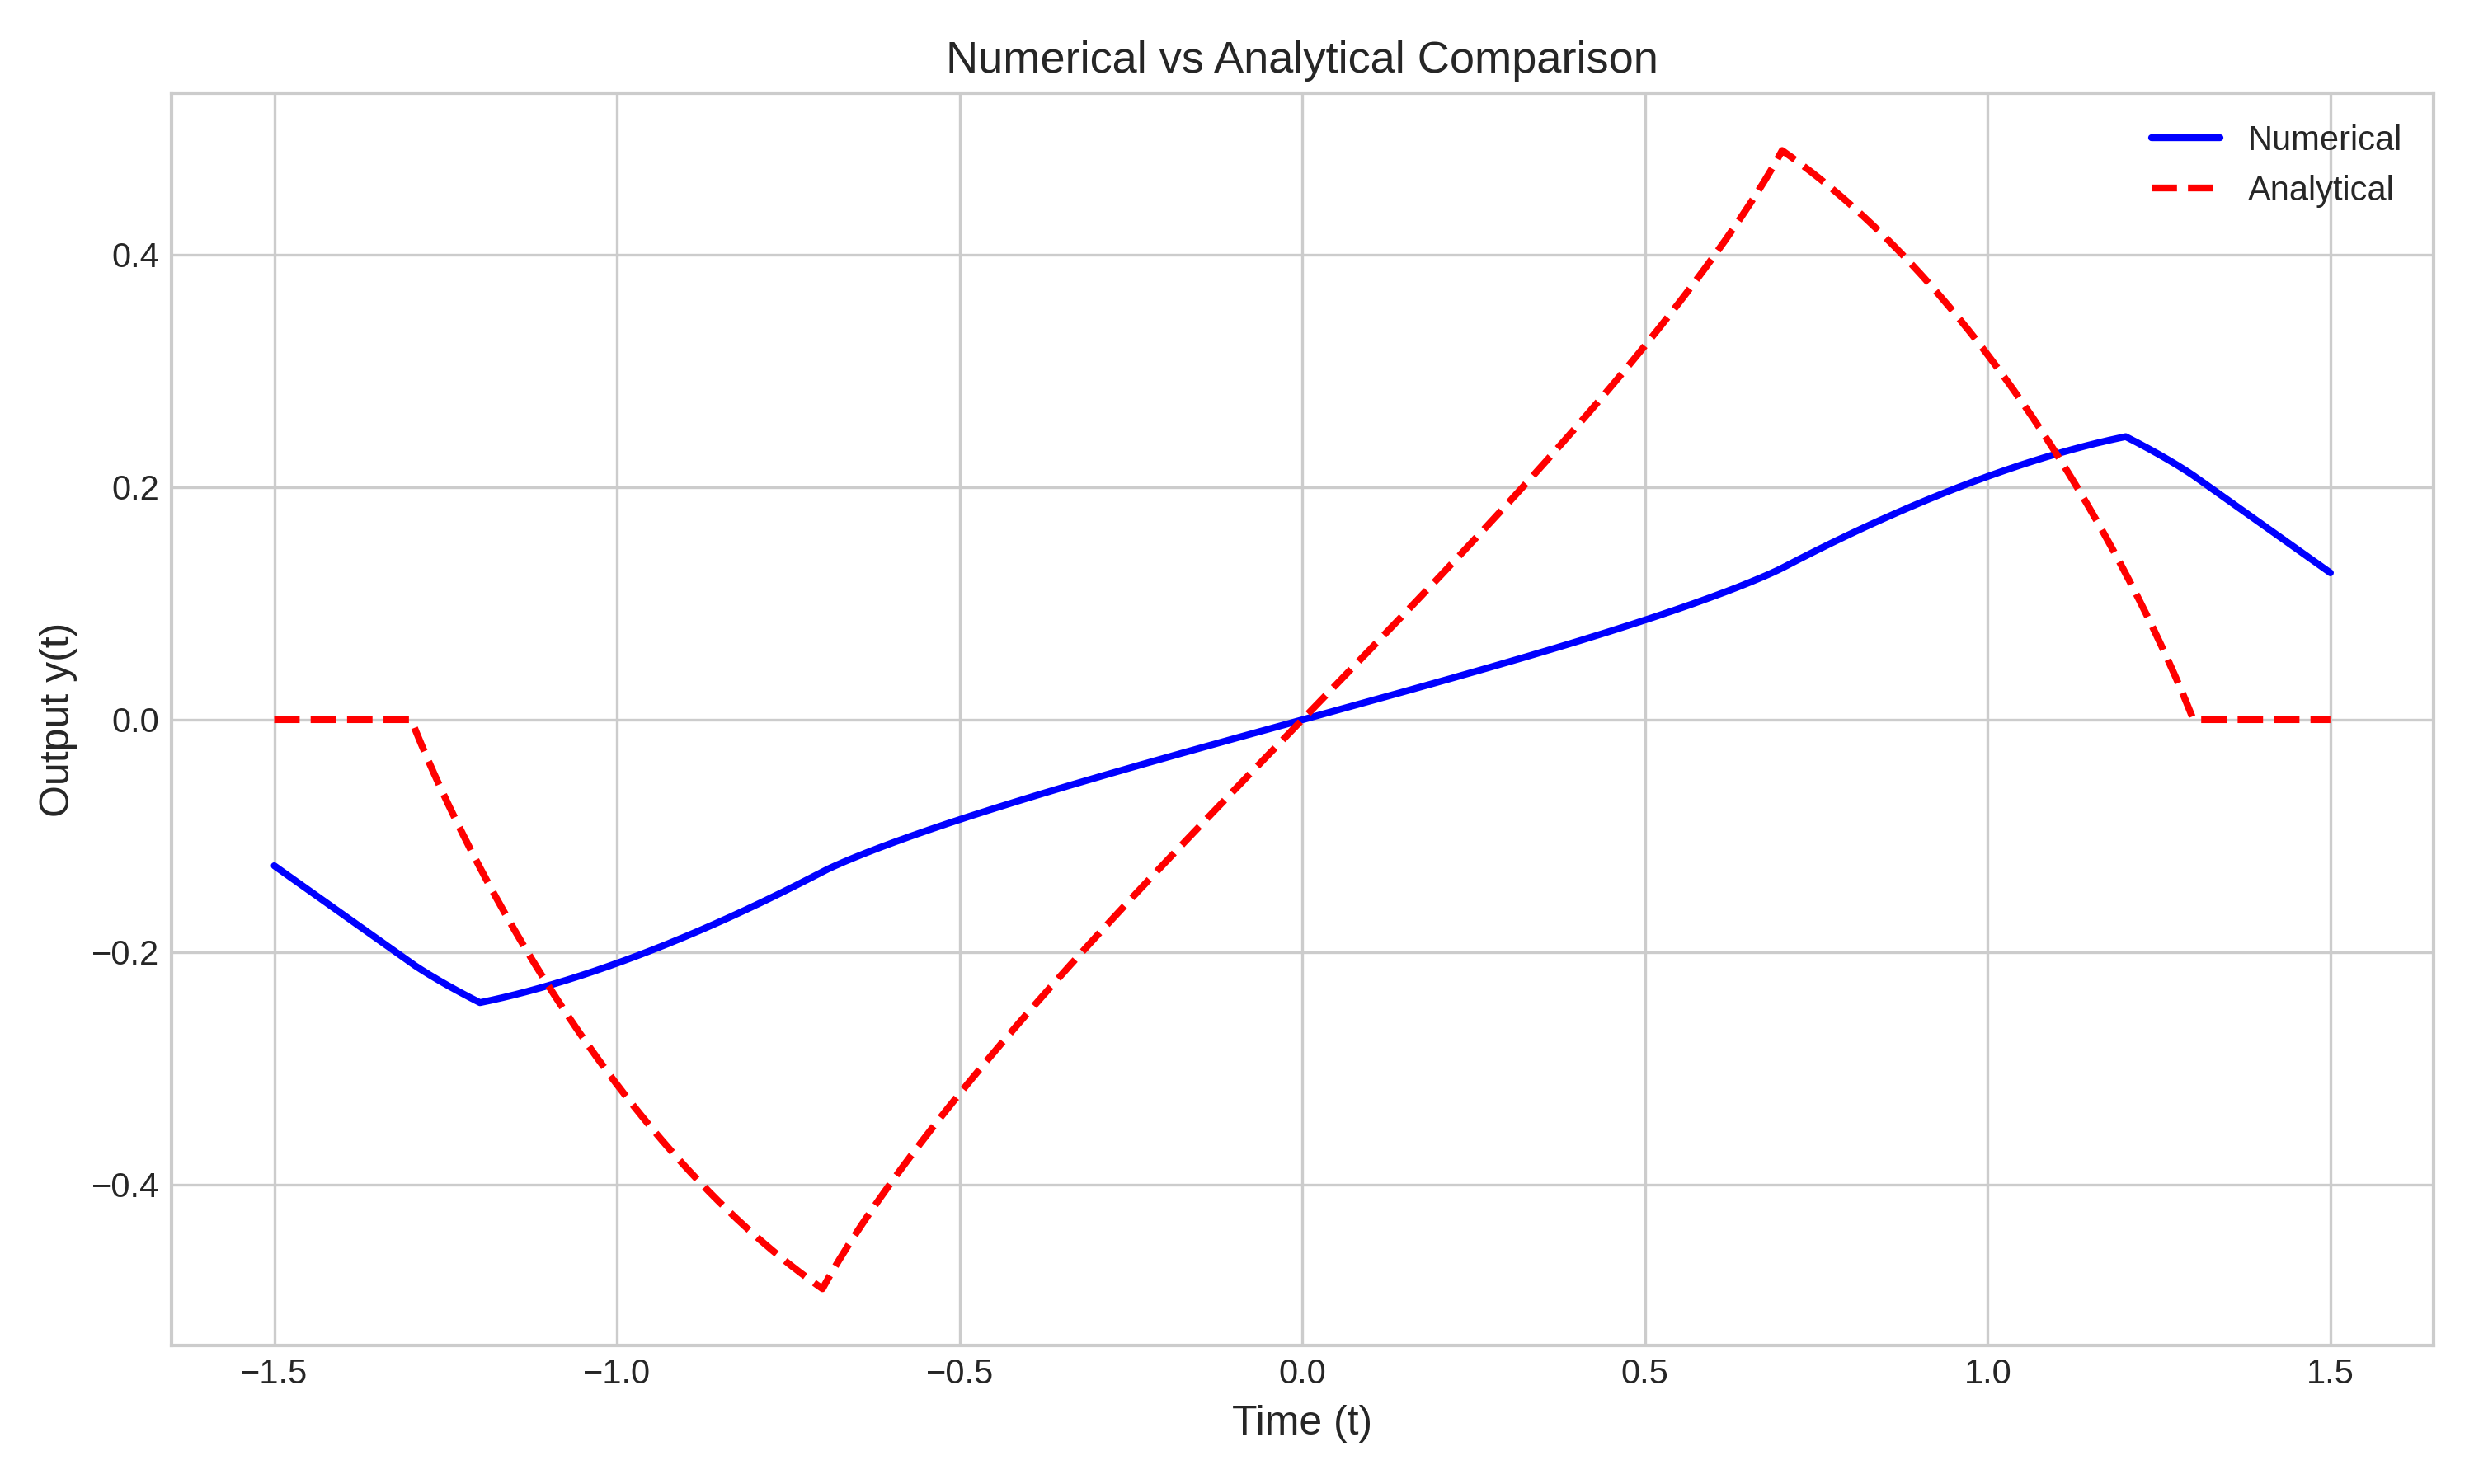
\includegraphics[width=0.85\textwidth]{codes/codes_sin_1_and_arcsin/figures/comparison.png}
    \caption{Numerical vs analytical comparison showing agreement in valid regions}
    \label{fig:comparison}
\end{figure}

Critical findings:
\begin{itemize}
\item Excellent agreement in central region $[-1+T, 1-T]$
\item Boundary discrepancies highlight numerical challenges
\item Analytical solution becomes singular at domain edges
\end{itemize}

\subsection{Conclusion}
This analysis demonstrates that while the arcsin function presents unique challenges for convolution operations, both analytical and numerical methods can provide valuable insights when properly implemented. The key findings include:

\begin{itemize}
\item Linear amplitude scaling with input signal magnitude
\item Direct relationship between kernel width and output amplitude
\item Importance of proper domain handling for arcsin function
\item Necessity of numerical methods for full-domain analysis
\end{itemize}

These results emphasize the importance of understanding domain constraints when working with nonlinear functions in signal processing applications.
